
\thispagestyle{empty}

\begin{center}
{\bf \em \huge Bayes{\Huge X}}

\vspace{0.5cm}

{\em \large Software for Bayesian Inference}

\vspace{0.5cm}

{\em Version 1.40}

\vspace{0.5cm}

\begin{figure}[h]
\begin{center}
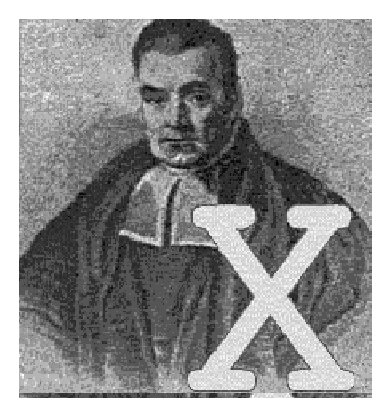
\includegraphics[scale=1.2]{grafiken/bayesicon.eps}
\end{center}
\end{figure}

\vfill

{\bf\sffamily \huge Reference Manual}

\vfill

\end{center}

\begin{table}[ht]
\begin{center}
\begin{tabular}{lll}
{\em developed at} & \hspace{1.5cm} & {\em developed by} \\
University of Munich & \hspace{1.5cm} & Andreas Brezger \\
Department of Statistics & \hspace{1.5cm} & Thomas Kneib \\
Ludwigstr. 33 & \hspace{1.5cm} & Stefan Lang \\
80539 Munich & \hspace{1.5cm} & \\
  & & \\
{\em with contributions by}  &  \hspace{1.5cm} &  {\em supported by} \\
Christiane Belitz&  \hspace{1.5cm} & Ludwig Fahrmeir (mentally) \\
Eva--Maria Fronk  & \hspace{1.5cm} & Leo Held (mentally) \\
Andrea Hennerfeind & \hspace{1.5cm} & German Science Foundation  \\
Manuela Hummel & \\
Alexander Jerak & \\
Petra Kragler & \\
Leyre Osuna Echavarr\'{\i}a& \\
\end{tabular}
\end{center}
\end{table}


\newpage

\subsection*{Acknowledgements}

The development of {\em BayesX} has been supported by grants from
the German National Science Foundation (DFG),
Sonderforschungsbereich 386.

Special thanks go to (in alphabetical order of first names):

{\em Dieter Gollnow} for computing and providing the map of Munich (a really hard job); \\
{\em Leo Held} for advertising the program; \\
{\em Ludwig Fahrmeir} for his patience with finishing the program
and for carefully
reading and correcting the  manual; \\
{\em Ngianga-Bakwin Kandala} for being the first user of the program (a really hard job); \\
{\em Samson Babatunde Adebayo} for carefully reading and correcting the manual; \\
{\em Ursula Becker} for carefully reading and correcting the
manual;

\subsection*{Licensing agreement} The authors of this software grant
to any individual or non-commercial organization the right to use
and to make an unlimited number of copies of this software. Usage
by commercial entities requires a license from the authors. You
may not decompile, disassemble, reverse engineer, or modify the
software. This includes, but is not limited to modifying/changing
any icons, menus, or displays associated with the software. This
software cannot be sold without written authorization from the
authors. This restriction is not intended to apply for connect
time charges, or flat rate connection/download fees for electronic
bulletin board services. The authors of this program accept no
responsibility for damages resulting from the use of this software
and make no warranty on representation, either express or implied,
including but not limited to, any implied warranty of
merchantability or fitness for a particular purpose. This software
is provided as is, and you, its user, assume all risks when using
it.

\vspace{0.5cm}

{\em BayesX} is available at {
\href{http://www.stat.uni-muenchen.de/~bayesx}{http://www.stat.uni-muenchen.de/\~{}bayesx}}

\newpage

\pdfbookmark[1]{Contents}{contents} \tableofcontents
\hypertarget{contents}{}


\newpage
